\begin{figure}[htb]
	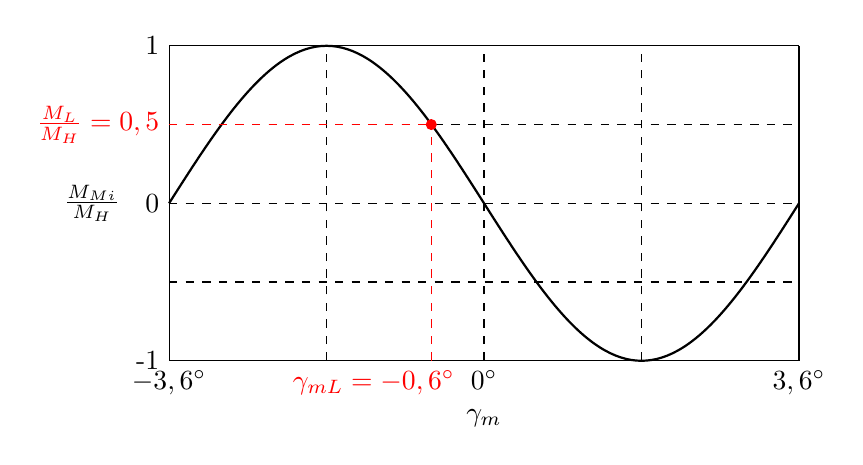
\begin{tikzpicture}
	
	% vertical axes
	\draw (0,-2) node [below] {$-3,6^\circ$} -- (0,2);
	\draw [dashed] (2,-2) -- (2,2);
	\draw [dashed] (4,-2) node [below] {$0^\circ$} -- (4,2);
	\draw  node [below] at (4,-2.5) {$\gamma_m$};
	\draw [dashed] (6,-2) -- (6,2);
	\draw (8,-2) node [below] {$3,6^\circ$} -- (8,2);
	
	% horizontal axes	
	\draw (0,-2) node [left] {-1} -- (8,-2);
	\draw [dashed] (0,-1) -- (8,-1);
	\draw [dashed] (0,0) node [left] {0} -- (8,0);
	\draw  node [left] at (-0.5,0) {$\frac{M_{Mi}}{M_H}$};
	\draw [dashed] (0,1) -- (8,1);
	\draw (0,2) node [left] {1} -- (8,2);
	
	% sine
    \draw[thick]
    (0,0) sin (2,2) cos (4,0) sin (6,-2) cos (8,0);	
	
    % additional information
    \draw [red, dashed] (0,1) node [left] {$\frac{M_L}{M_H} = 0,5$} -- (3.33,1);
    \fill [red] (3.33,1) circle [radius=2pt];
    \draw [red, dashed] (3.33,-2) -- (3.33,1);
    \draw [red] node [below] at (2.6,-2) {$\gamma_{mL} = -0,6^\circ$};
	
	\end{tikzpicture}
	\caption{Drehmomentverlauf}
	\label{dia:aufg3b_drehmoment}
\end{figure}